\documentclass[3p,review]{elsarticle}

\usepackage{lineno,hyperref}
%\usepackage{amsmath}
%\usepackage{arydshln}
\usepackage{subcaption}
%\usepackage{subfigure}
\usepackage{comment,color}


\usepackage{graphicx,amsfonts,url,multirow}
%\usepackage[cmex10]{amsmath}
\modulolinenumbers[5]

\journal{Information Fusion}

\newcommand{\TODO}{\textbf{TODO}}

%%%%%%%%%%%%%%%%%%%%%%%%%%%%%%%%%%%%%%%%%%%%%%%%%%%%%%%%%%%%%%%%%%%%%%%%%%%%%%%%%%%%%%%%%

\begin{document}

\begin{frontmatter}

\title{Big Data Analytics: A Tutorial on Information Process Fusion with MapReduce}

\author[grx]{Sergio Ram\'irez\corref{cor1}}
\ead{sramirez@decsai.ugr.es}

\author[grx]{Alberto Fern\'andez}
\ead{alberto@decsai.ugr.es}

\author[grx]{Salvador Garc\'ia}
\ead{salvagl@decsai.ugr.es}

\author[grx]{Francisco Herrera}
\ead{herrera@decsai.ugr.es}

\address[grx]{Department of Computer Science and Artificial Intelligence, University of Granada, Granada, Spain}
%\address[kau]{Faculty of Computing and Information Technology - North Jeddah, King Abdulaziz University (KAU), Jeddah, Saudi Arabia}


\cortext[cor1]{Corresponding author. Tel:+34-958-240598; Fax: +34-958-243317}

\begin{abstract}

\TODO

%In this paper we aim at presenting the first outcomes in this framework, and to analyze the behavior of standard solutions to address imbalanced classification in Big Data problems. The features of these recent approaches, and the experimental results obtained throughout this work, will allow us to determine the current state of this area of research and to provide a discussion on the future directions. 

\end{abstract}

\begin{keyword}
Big Data Analytics, MapReduce, Information Fusion, Spark, Machine Learning
\end{keyword}

\end{frontmatter}

\section{Introduction}\label{sec:intro}

\TODO

In order to address all these objectives, this paper is organized as follows. First, Section \ref{sec:mr} presents an introduction on the MapReduce programming framework, also stressing some alternatives for Big Data processing. Section \ref{sec:techno} includes an overview on those technologies currently available to address Big Data problems from a distributed perspective. Section \ref{sec:fusion} presents the core of this paper, analyzing the different design options for developing Big Data analytics algorithms regarding how the partial data and models are aggregated. Then, we show a case study in Section \ref{sec:exp} to contrast the capabilities regarding scalability of the different approaches previously introduced. Finally, Section \ref{sec:conclusions} summarizes and concludes this paper.

\section{MapReduce as Information Process Fusion}\label{sec:mr}

INTRO

\subsection{MR}\label{subsec:mr}

The rapid growth and influx of data from private and public sectors has popularized the notion of ``Big data \cite{Fer14}''. The surge in Big Data has led to the development of custom models and algorithms that are able to extract significant value and insight in different areas such as medical, health care, business, management and so on \cite{Kam14,Chen14,Wu14}.

In order to to provide robust and scalable solutions, new research paradigms and developmental tools have been made available. These frameworks have been designed to ease both the storage necessities and the processing of Big Data problems \cite{Fer14}. 

The MapReduce execution environment \cite{Dea08} is the most common framework used in this scenario. Being a privative tool, its open source counterpart, known as Hadoop, has been traditionally used in academia research \cite{Whi15-Hadoop}. It has been designed to allow distributed computations in a transparent way for the programmer, also providing a fault-tolerant execution scheme. To take advantage of this scheme, any algorithm must be divided into two main stages: Map and Reduce. The first one is devoted to split the data for processing, whereas the second collects and aggregates the results.

Additionally, the MapReduce model is defined with respect to an essential data structure: the $<$key,value$>$ pair. The processed data, the intermediate and final results work in terms of $<$key,value$>$ pairs. To summarize its procedure, Figure \ref{fig:mapreduce} illustrates a typical MapReduce program with its \textit{Map} and \textit{Reduce} steps. The terms $k_i:v_j$ refer to the key and value pair that are computed within each Map process. Then, values are grouped linking them to the same key, i.e. $k_i:v_j,\ldots, v_h$, and feed to the same Reduce process. Finally, values are aggregated with any function within the Reduce process to obtain the final result of the algorithm.

%\begin{comment}
\begin{figure}[!ht]
\centering \resizebox{0.75\textwidth}{!}{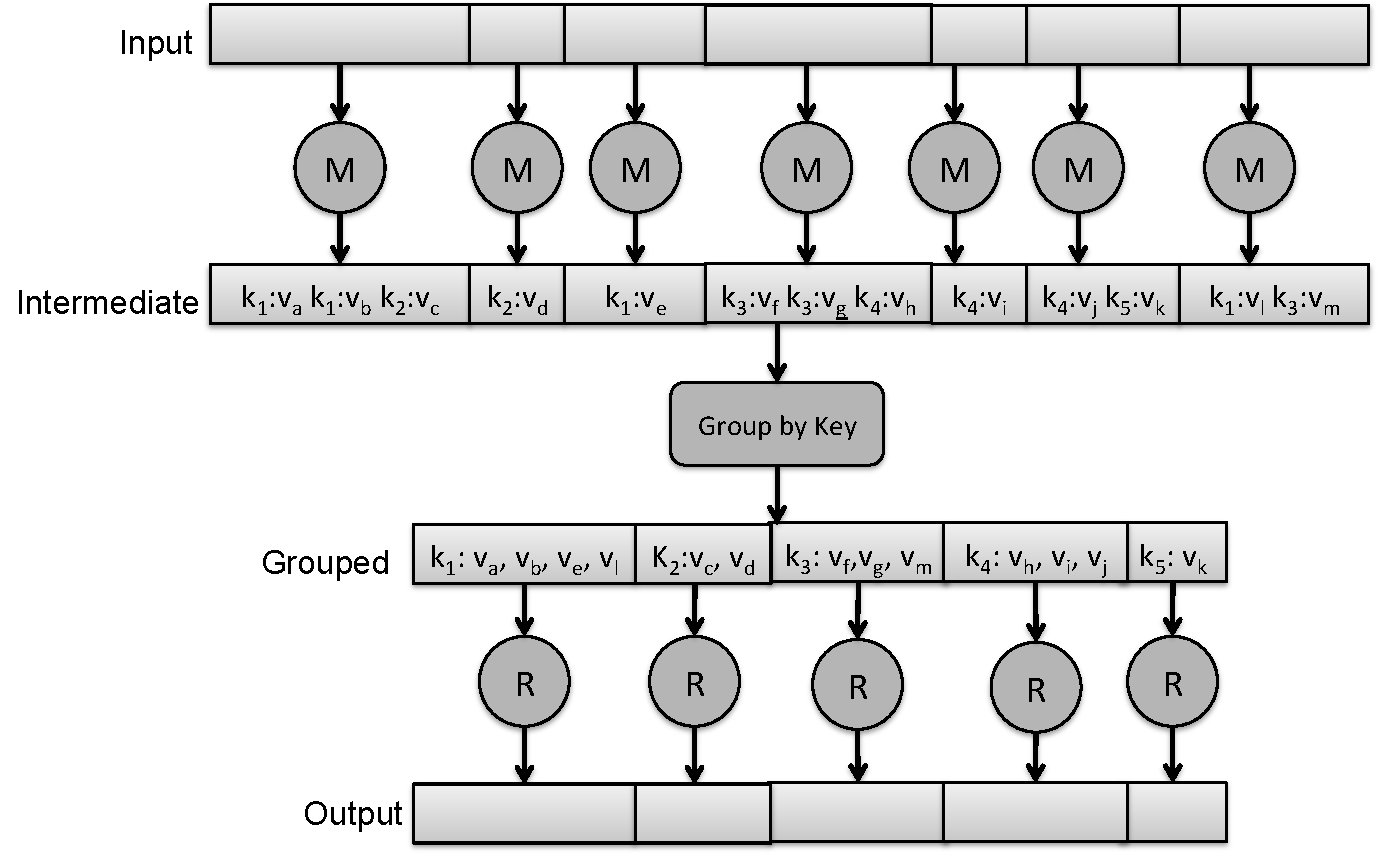
\includegraphics{mapreduce}} \caption{The MapReduce programming model.}
\label{fig:mapreduce}
\end{figure}
%\end{comment}

From this initial model, more recent alternative frameworks have arisen to provide more efficient computations for iterative process, which are the basis for any Machine Learning algorithm. Among them, Apache Spark \cite{Zaharia12,Zaharia10} is clearly emerging as a more commonly embraced platform for implementing Machine Learning solutions that scale with Big Data.

\subsection{Alternatives}\label{subsec:altMR}

\TODO

\section{Big Data Technologies for Analytics}\label{sec:techno}

\TODO

\subsubsection{Hadoop}\label{subsec:hadoop}

\TODO

\subsubsection{Spark}\label{subsec:spark}

Spark\cite{Zaharia12,Zaharia10} \footnote{\url{http://spark.apache.org/}} has been developed to overcome data reuse across multiple computations. It supports iterative applications, while retaining the scalability and fault tolerance of MapReduce, supporting in-memory processes. It is implemented in the functional programming language Scala and has further programming interfaces in Java, Python and the declarative query language SparkSQL.

Spark rests upon two main concepts: resilient distributed datasets (RDD), which hold the data objects in memory, and transformations or actions that are performed on the datasets in parallel.

RDDs are a collection of distributed items, with read-only-mode and fault-tolerant. As stated above, these data structures allow users making intermediate results to persist in memory, as well as controlling their partitioning to optimize data placement, and also manipulating them using a rich set of operators.

These operators are based on coarse-grained transformations. Specifically, there are 20 transformations and 12 actions usable. The difference between the two kinds of operators is that transformations are functions to generate and manipulate RDDs out of input files or other RDDs, whereas actions can only be used on RDDs to produce a result set in the driver program or write data to the file system\cite{Zaharia12}.

In order to manage data objects within the algorithms developed under Spark, two API are available in current version 1.6.0. On the first hand, DataFrame API, which is clearly the most stable option and therefore it offers the best performance. On the other hand, an API simply named as Dataset may be used also. However, being the most recent add to this framework, it does not yet leverage the additional information it has, and it can be slower than RDDs. It is expected to be fully developed and improved for Spark version 2.0.

It is worth to point out that Spark implements a Machine Learning library known as MLlib\footnote{\url{http://spark.apache.org/docs/latest/mllib-guide.html}}, included within the MLBase platform \cite{Kra13}. MLlib currently supports common types of machine learning problem settings, as well as associated tests and data generators. It includes binary classification, regression, clustering and collaborative filtering, as well as an underlying gradient descent optimization primitive. Finally, Mahout \cite{Owe11}, maybe the most well-known Machine Learning library for Big Data, has recently announced its migration to Spark, due to the good properties of this framework for the execution of this type of algorithms. Neither of them support any fuzzy modeling algorithm yet.

\subsubsection{Flink}\label{subsec:flink}

The Flink framework\footnote{\url{http://flink.apache.org/}} has its origins in the Stratosphere project \cite{Alexandrov14,Hues12}. The main idea behind this model is the optimization of execution plans, which is based on basic technologies from relational database systems. It is written in Java, but it also supports Scala and Python languages. It avoids the use of a declarative query language with aims at simplifying the development of applications for those users with less programming experience.

The Apache Flink framework currently provides 17 functions for data transformation, which are known as PACT operators, which are quite similar to that of the Spark framework. The main difference is based on two unique iteration operators, namely bulkIteration and deltaIteration. The former operator employ the whole dataset in every run, whereas the latter divides the data in a workset and solution set. One of the advantages of these iterators is that fewer data has to be computed and sent between nodes  \cite{EwenTKM12}. In accordance to the former, these are better suited for an efficient implementation of both machine learning and data mining algorithms, supporting also data stream processing.

As stated at the beginning, one of the most interesting features of the Flink framework is known as the PACT optimizer. It creates several semantically equivalent execution plans by reordering the PACT operators based on code analysis and data access conflicts \cite{Alexandrov14,Hues12}. The physical optimization chooses efficient strategies for data transport and operator execution on specific nodes. A cost-based strategy selects the most efficient plan based on criteria like network or storage I/O costs.

Finally, the Flink ecosystem also provides a Machine Learning library, FlinkML\footnote{\url{https://ci.apache.org/projects/flink/flink-docs-release-0.10/libs/ml/}}, which includes several data preprocessing, supervised learning, and recommender systems. It is still at a preliminary stage, but it is expected to add new algorithms in a short future.

\section{Big Data Analytics on Fusion Process}\label{sec:fusion}

\TODO

\subsection{Direct fusion of models: ensemble approach}\label{subsec:ensemble}

\TODO

\subsection{Approximate fusion of models: aggregation of partial systems}\label{subsec:submodels}

\TODO

\subsection{Exact fusion for scalable models: distributed data and models' partition}\label{subsec:exact}

\TODO

\section{Practical Study on XXX}\label{sec:exp}

\TODO



\section{Concluding Remarks}\label{sec:conclusions}

\TODO

\section*{Acknowledgments}\label{sec:ack}

This work have been partially supported by the Spanish Ministry of Science and Technology under projects TIN2014-57251-P and TIN2015-68454-R; and the Foundation BBVA project 75/2016 BigDaPTOOLS.
%\newline

%\noindent\appendix{\textbf{Bibliography}}\label{sec:biblio}

\bibliographystyle{elsarticle-num}
\bibliography{cloud}

\end{document}
